\documentclass[10pt,twocolumn,letterpaper]{article}
\usepackage[top=0.8in,bottom=0.8in,left=0.72in,right=0.72in,columnsep=0.27in,headheight=12pt,headsep=14pt]{geometry}
\usepackage[T1]{fontenc}
\usepackage[utf8]{inputenc}
\usepackage{newtxtext,newtxmath}
\usepackage[scaled=0.9]{inconsolata}
\usepackage[final,tracking=true]{microtype}
\usepackage{graphicx,booktabs,array,xcolor,enumitem,titlesec,fancyhdr,caption,float,etoolbox}
\PassOptionsToPackage{hyphens}{url}
\usepackage[authoryear,round,sort&compress]{natbib}
\usepackage[colorlinks=true,linkcolor=ink,citecolor=gwgreen,urlcolor=gwgreen,pdftitle={Seeing a War Without Standing in It},pdfauthor={Poon Thiengburanathum; Non Arkaraprasertkul},pdfsubject={Open-data situational awareness of the 2026 Gulf conflict},pdfkeywords={open-source intelligence; AIS; ADS-B; conflict; observability; Hormuz}]{hyperref}
\definecolor{ink}{HTML}{191712}\definecolor{ink2}{HTML}{6F6C63}\definecolor{gwgreen}{HTML}{1F6E43}\definecolor{gwred}{HTML}{A23A26}\definecolor{rule}{HTML}{D2CFC5}
% generated by research/scripts/make_tex_inputs.py -- do not edit
\newcommand{\NSessions}{212}
\newcommand{\BrentBase}{72.48}
\newcommand{\BrentFirst}{7.3}
\newcommand{\BrentFive}{27.9}
\newcommand{\BrentTwenty}{55.3}
\newcommand{\BrentPeakPct}{63.3}
\newcommand{\BrentPeakClose}{118.35}
\newcommand{\BrentLatestPct}{43.6}
\newcommand{\BrentLatest}{104.06}
\newcommand{\VolPre}{2.19}
\newcommand{\VolPost}{4.07}
\newcommand{\SPPre}{0.76}
\newcommand{\SPPost}{0.83}
\newcommand{\CorrPre}{$-$0.43}
\newcommand{\CorrPost}{$-$0.75}
\newcommand{\CorrPreCI}{$-$0.66 to $-$0.13}
\newcommand{\CorrPostCI}{$-$0.81 to $-$0.67}
\newcommand{\SpreadPre}{4.69}
\newcommand{\SpreadPost}{6.35}
\newcommand{\SpreadMax}{16.97}
\newcommand{\PctileFive}{99.7}
\newcommand{\PctileTwenty}{99.7}
\newcommand{\LogTwenty}{44.0}
\newcommand{\UkrTwenty}{25.6}
\newcommand{\WarTwenty}{55.3}
\newcommand{\UkrSixty}{15.7}
\newcommand{\WarSixty}{37.4}
\newcommand{\AuditClaim}{140}
\newcommand{\AuditClose}{81.40}
\newcommand{\AuditHigh}{126.10}
\newcommand{\AuditHighDate}{30 April}
\newcommand{\GoldAbs}{23.2}
\newcommand{\FrontlineTwentyAbs}{11.3}
\newcommand{\LufthansaAbs}{17.8}
\newcommand{\AFAbs}{11.5}
\newcommand{\TTFLatest}{186.6}
\newcommand{\DeltaLatest}{26.8}
\newcommand{\LufthansaLatest}{-17.8}
\newcommand{\AFLatest}{-11.5}
\newcommand{\FrontlineLatest}{38.2}
\newcommand{\MaerskLatest}{46.7}
\newcommand{\RangeStart}{2 January 2026}
\newcommand{\RangeEnd}{4 November 2026}
\newcommand{\GulfPre}{74.3}
\newcommand{\GulfPost}{20.9}
\newcommand{\GulfRatio}{28}
\newcommand{\GulfLo}{26}
\newcommand{\GulfHi}{30}
\newcommand{\GulfTankPre}{19.7}
\newcommand{\GulfTankPost}{5.4}
\newcommand{\GulfTankRatio}{27}
\newcommand{\OmanRatio}{57}
\newcommand{\RedRatio}{83}
\newcommand{\RedLo}{73}
\newcommand{\RedHi}{92}
\newcommand{\MedRatio}{91}
\newcommand{\CtrlRatio}{98}
\newcommand{\GulfMar}{25}
\newcommand{\GulfMay}{19}
\newcommand{\GulfJul}{36}
\newcommand{\GulfOct}{31}
\newcommand{\RedExJeddah}{90}
\newcommand{\JeddahJun}{102}
\newcommand{\JeddahOct}{13}
\newcommand{\RedOct}{44}
\newcommand{\PortDaysPre}{423}
\newcommand{\PortDaysPost}{244}
\newcommand{\AisTotal}{68,680}
\newcommand{\AisFresh}{12,043}
\newcommand{\AisFreshPct}{17.5}
\newcommand{\AisMedianAge}{170}
\newcommand{\AisPnineAge}{2,219}
\newcommand{\AisSnaps}{4}
\newcommand{\AisSpanMin}{81}
\newcommand{\AisFreshMin}{17.5}
\newcommand{\AisFreshMax}{17.6}
\newcommand{\HormuzAll}{1,110}
\newcommand{\HormuzFresh}{0}
\newcommand{\HormuzFreshPct}{0.0}
\newcommand{\PGulfAll}{1,171}
\newcommand{\PGulfFresh}{1}
\newcommand{\PGulfFreshPct}{0.1}
\newcommand{\GOmanAll}{37}
\newcommand{\GOmanFresh}{0}
\newcommand{\GOmanFreshPct}{0.0}
\newcommand{\RedSeaAll}{0}
\newcommand{\RedSeaFresh}{0}
\newcommand{\RedSeaFreshPct}{--}
\newcommand{\BabElAll}{0}
\newcommand{\BabElFresh}{0}
\newcommand{\BabElFreshPct}{--}
\newcommand{\SuezAll}{681}
\newcommand{\SuezFresh}{26}
\newcommand{\SuezFreshPct}{3.8}
\newcommand{\MalaccaAll}{8,357}
\newcommand{\MalaccaFresh}{353}
\newcommand{\MalaccaFreshPct}{4.2}
\newcommand{\NSeaAll}{3,369}
\newcommand{\NSeaFresh}{1,914}
\newcommand{\NSeaFreshPct}{56.8}
\newcommand{\BalticAll}{2,206}
\newcommand{\BalticFresh}{936}
\newcommand{\BalticFreshPct}{42.4}
\newcommand{\CapeAll}{1,922}
\newcommand{\CapeFresh}{175}
\newcommand{\CapeFreshPct}{9.1}
\newcommand{\FirmsRows}{271,252}
\newcommand{\FirmsDays}{6}
\newcommand{\FirmsFrom}{28 October}
\newcommand{\FirmsTo}{2 November 2026}
\newcommand{\FirmsGulfChronic}{19}
\newcommand{\FirmsGulfCells}{611}
\newcommand{\FirmsGulfBig}{3}
\newcommand{\FirmsOtherChronicMax}{4}
\newcommand{\AirN}{8}
\newcommand{\AirME}{405}
\newcommand{\AirEU}{2,293}
\newcommand{\AirSEA}{464}
\newcommand{\AirMELo}{344}
\newcommand{\AirMEHi}{452}
\newcommand{\DensUAE}{50.0}
\newcommand{\MeanUAE}{35.8}
\newcommand{\DensIran}{0.0}
\newcommand{\MeanIran}{0.6}
\newcommand{\DensIraq}{0.0}
\newcommand{\MeanIraq}{0.0}
\newcommand{\DensEgypt}{0.5}
\newcommand{\MeanEgypt}{4.6}
\newcommand{\DensSaudi}{0.7}
\newcommand{\MeanSaudi}{13.0}
\newcommand{\DensTurkey}{12.0}
\newcommand{\MeanTurkey}{93.6}
\newcommand{\DensIsrael}{20.9}
\newcommand{\MeanIsrael}{4.6}
\newcommand{\DensJordan}{10.9}
\newcommand{\MeanJordan}{9.8}
\newcommand{\DensSyria}{5.3}
\newcommand{\MeanSyria}{9.9}
\newcommand{\AirEUMedian}{28.6}
\newcommand{\AirSEAMedian}{6.1}

\urlstyle{same}\Urlmuskip=0mu plus 2mu\relax
\def\UrlBreaks{\do\/\do-\do_\do.\do?\do=\do\&\do\#}

% ---------- typography
\setlength{\parindent}{1.1em}\setlength{\parskip}{0pt}\linespread{1.04}
\setlist{nosep,leftmargin=1.2em,itemsep=2pt}
\titleformat{\section}{\normalfont\large\bfseries\color{ink}}{\thesection}{0.6em}{}[\vspace{-0.45em}{\color{rule}\titlerule}]
\titleformat{\subsection}{\normalfont\normalsize\bfseries\itshape\color{ink}}{\thesubsection}{0.5em}{}
\titlespacing*{\section}{0pt}{1.3ex plus .4ex minus .2ex}{0.9ex}
\titlespacing*{\subsection}{0pt}{1.0ex plus .3ex minus .2ex}{0.4ex}
\captionsetup{font=small,labelfont={bf},labelsep=period,justification=raggedright,singlelinecheck=false,skip=3pt}
\renewcommand{\arraystretch}{1.08}
\setlength{\tabcolsep}{4pt}
\setlength{\textfloatsep}{9pt plus 2pt minus 2pt}\setlength{\floatsep}{8pt plus 2pt minus 2pt}\setlength{\intextsep}{8pt}
\setlength{\bibsep}{1.5pt}
\renewcommand{\bibfont}{\footnotesize}
\newcommand{\pct}{\%}
\newcommand{\kbox}[1]{\par\medskip\noindent{\color{gwgreen}\rule{\linewidth}{0.7pt}}\par\vspace{2pt}\noindent #1\par\vspace{1pt}{\color{rule}\rule{\linewidth}{0.4pt}}\par\medskip}

\pagestyle{fancy}\fancyhf{}
\fancyhead[L]{\footnotesize\color{ink2}Thiengburanathum \& Arkaraprasertkul}
\fancyhead[R]{\footnotesize\color{ink2}Seeing a War Without Standing in It}
\fancyfoot[C]{\footnotesize\color{ink2}\thepage}
\renewcommand{\headrulewidth}{0.3pt}\renewcommand{\headrule}{\hbox to\headwidth{\color{rule}\leaders\hrule height \headrulewidth\hfill}}
\fancypagestyle{first}{\fancyhf{}\fancyhead[L]{\footnotesize\bfseries\color{gwgreen}PREPRINT\ \ \normalfont\color{ink2}Not peer reviewed \textperiodcentered{} v1.0 \textperiodcentered{} 4 November 2026}\fancyhead[R]{\footnotesize\color{ink2}globalmonitor.nonarkara.org}\fancyfoot[C]{\footnotesize\color{ink2}\thepage}\renewcommand{\headrulewidth}{0.3pt}}

\begin{document}
\twocolumn[{%
\thispagestyle{first}
\vspace{-0.2em}
{\raggedright\fontsize{24}{27}\selectfont\bfseries\color{ink} Seeing a War Without Standing in It\par}
\vspace{5pt}
{\raggedright\fontsize{11.5}{14.5}\selectfont\itshape\color{ink2} What open ships, planes, satellites and markets reveal about the 2026 Gulf conflict, and where they go blind\par}
\vspace{9pt}
{\raggedright\large Poon Thiengburanathum\textsuperscript{1,2}\quad\quad Non Arkaraprasertkul\textsuperscript{3,*}\par}
\vspace{3pt}
{\raggedright\footnotesize\color{ink2}\textsuperscript{1}Faculty of Engineering, Chiang Mai University\ \ \textperiodcentered\ \ \textsuperscript{2}Research and Innovation Acceleration Agency for Competitiveness and Area Development (RCAD)\ \ \textperiodcentered\ \ \textsuperscript{3}Digital Economy Promotion Agency (depa), Thailand\ \ \textperiodcentered\ \ \textsuperscript{*}Correspondence: \href{mailto:non.ar@depa.or.th}{non.ar@depa.or.th}\par}
\vspace{4pt}{\color{rule}\rule{\textwidth}{0.5pt}}\vspace{2pt}
}]

\noindent\textbf{Abstract.}\ Journalists in conflict zones are dying at record rates: 129 press members were killed in 2025, by one count. Most of us will never go, and would help little if we did. Can we understand a war from outside, safely, with what is already public? We built an open observatory, GlobalWatch, that reads five \emph{witnesses} that need nobody's permission: ship transponders, aircraft transponders, thermal satellites, markets and aviation regulators. We tested it on the conflict that began on 28 February 2026. Money and ports speak clearly. Brent rose \BrentPeakPct\pct\ to its peak close, and its 20-session move sits at the \PctileTwenty\textsuperscript{th} percentile of all such moves since 2015; port calls inside the Persian Gulf fell to \GulfRatio\pct\ of their earlier rate (95\pct\ CI \GulfLo--\GulfHi\pct), while control ports held at \CtrlRatio\pct. Free transponder feeds go blind exactly where it matters: only \AisFreshPct\pct\ of \AisTotal\ vessel positions were under six hours old, none lay in the Red Sea, and the Gulf was quieter than every other lane we measured, so a silence there cannot be told apart from a coverage gap. Our own platform also erred: a hand-written milestone claimed \$\AuditClaim\ Brent on 4 March, when the close was \$\AuditClose, and a composite gauge read ``LOW'' while three of its four inputs were offline. The contribution is not a sharper eye but an honest one: every reading should travel with a measure of what could have been seen. Code, data and scripts are open.

\smallskip\noindent\textbf{Key points.}
\begin{itemize}
\item \textbf{Seen clearly:} prices and port calls moved at once, far outside normal range, and independent sources agree.
\item \textbf{Seen poorly:} free ship and aircraft feeds cannot tell an empty sea from an unheard one.
\item \textbf{Seen wrongly, by us:} three errors in our own dashboard, found by auditing it with the same method.
\item \textbf{The rule:} never show a silence without showing how well the sensor could hear.
\end{itemize}

\section{The question}
Journalists are dying faster than ever. The Committee to Protect Journalists counted 129 press members killed in 2025, the most in its records, after 124 in 2024 as first reported \citep{cpj2026report,cpj2025report}. Most of us have no combat experience. Going would add one more body to a war zone, not one more witness to it.

So the question is practical. From outside, can we understand what is happening? Do liners and cargo ships still move? Do aircraft still fly, and which skies do they refuse? What do prices say? What burns? And can a small team, without permissions or budgets, answer these in a way that anyone can use today?

Two things make the question harder than it looks. First, reporting is itself a sensor, and it has eyesight. It sees what reporters can reach and editors choose to print \citep{earl2004newspaper,weidmann2016reporting}. Event datasets built on reporting inherit that eyesight \citep{raleigh2010acled,sundberg2013ucdp,leetaru2013gdelt}. Second, the machines that do not need reporters have eyesight too. A ship is a loud object: it announces itself every few seconds to anyone who listens. Whether anyone listens is another matter.

Our answer, the most important thing first: \emph{we can see that something changed, fast and cheaply, by reading systems that cannot lie cheaply, namely money, ports and regulators. We often cannot see why. In some places we cannot see at all, and the instrument will not say so unless it is made to.}

We make four contributions. (i) An open observatory that reads five independent witnesses. (ii) An \emph{observability audit}: a procedure for deciding whether an empty cell on a map is a quiet place or a deaf receiver. (iii) Evidence from the first eight months of the 2026 Gulf conflict. (iv) An audit of our own platform, which found three errors; we report them because the method is only credible if it is turned on its author.

\section{Related work}
\textbf{Open-source investigation} turned public traces into evidence long before this war \citep{higgins2021bellingcat}. \textbf{Conflict event data} (ACLED, UCDP, GDELT) code reports into counts and coordinates \citep{raleigh2010acled,sundberg2013ucdp,leetaru2013gdelt}; their known weakness is that reporting is uneven across space and time \citep{weidmann2016reporting}. \textbf{Remote sensing} sees without reporters: nightlights tracked the Syrian crisis \citep{li2014nightlights}, airborne sampling measured the Kuwait oil-fire smoke \citep{hobbs1992kuwait}, and thermal sensors now detect fire at 375\,m \citep{schroeder2014viirs}; \citet{witmer2015remote} reviews the field. The environmental toll of the Gaza war has been assessed the same way \citep{unep2024gaza}.

\textbf{Transponders.} Ship AIS reveals fisheries at global scale \citep{kroodsma2018fisheries}, satellite imagery finds the fleets that switch it off \citep{park2020darkfleets}, and AIS has been turned into trade nowcasts \citep{cerdeiro2020seaborne}. Aircraft ADS-B, collected by volunteer receivers, produced research-grade air-traffic data \citep{schafer2014opensky,strohmeier2021opensky}. Since flight MH17 was shot down over Ukraine \citep{dsb2015mh17}, civil aviation authorities have published conflict-zone guidance \citep{icao2018doc10084,easa2026czib}. \textbf{Markets} price geopolitical risk \citep{caldara2022gpr} and distinguish oil shocks by cause \citep{kilian2009oil}. \textbf{Dashboards} can inform in real time \citep{dong2020covid}, and forecasting war is hard \citep{cederman2017predicting,hegre2019views}, so we do not forecast here.

What is missing is a single frame that puts these channels side by side \emph{and} measures how well each could hear. That is the gap we fill.

\section{Method}
\subsection{Five witnesses}
Table~\ref{tab:witness} lists the witnesses. We chose them because each is produced by a system with its own purpose, so none was written to persuade us. Planes squawk to avoid collisions; ships broadcast to avoid collisions; satellites pass on their own schedule; markets clear because someone pays; regulators publish because liability demands it.

\begin{table*}[t]
\centering\small
\caption{The five witnesses. Every source is public; none required an agreement or a paid key for the analyses reported here.}\label{tab:witness}
\begin{tabular}{@{}>{\raggedright\arraybackslash}p{2.2cm}>{\raggedright\arraybackslash}p{3.6cm}>{\raggedright\arraybackslash}p{4.6cm}>{\raggedright\arraybackslash}p{1.9cm}>{\raggedright\arraybackslash}p{3.9cm}@{}}
\toprule
Witness & What it hears & Source used here & Cadence & Where it is deaf\\\midrule
Ships & AIS positions; port calls & Axiom Overwatch snapshot \citep{overwatch}; PortWatch daily port calls \citep{portwatch,arslanalp2021imf} & minutes; daily & Beyond receivers; spoofing; transponders off\\
Aircraft & ADS-B state vectors & OpenSky anonymous API \citep{opensky}; adsb.lol in the dashboard \citep{adsblol} & seconds & Receiver geometry; many military aircraft are silent\\
Heat & VIIRS 375\,m active-fire detections & NASA FIRMS open CSV \citep{firms} & about 2 passes a day per satellite & Cloud; industrial flares; no attribution\\
Money & Daily closes of 20 assets; oil flows & Yahoo Finance chart endpoint \citep{yahoofinance}; EIA flows \citep{eia2026steo} & daily & Causes are confounded\\
Rules & Airspace conflict bulletins & EASA CZIB list \citep{easa2026czib} & event-driven & Institutional lag and politics\\\bottomrule
\end{tabular}
\end{table*}

\subsection{Study design}
The event is the first strikes on Saturday 28 February 2026; the last pre-war close is 27 February. For prices we use \NSessions\ daily sessions from \RangeStart\ to \RangeEnd. For port calls we compare a pre-window (1 January 2025 to 27 February 2026, \PortDaysPre\ days) with a post-window (1 March to 30 October 2026, \PortDaysPost\ days), against control ports (Singapore, Rotterdam) that are far from the conflict. For transponders and heat we take cross-sections on 4 November 2026. The design is descriptive. It is one event with many confounders, and we make no causal claim.

\subsection{The observability audit}
A silence informs only if the sensor could have heard. For each channel we therefore measure, next to the reading, a proxy for what could have been seen. For AIS: the \emph{age} of each vessel's last position, with a six-hour threshold for ``currently at sea''. For ADS-B: occupancy of well-covered neighbours and non-conflict countries as a contrast. For heat: \emph{persistence}, meaning how many days the same 1\,km cell lights up, which separates chronic sources (flares, kilns) from transient ones. For all: cross-channel agreement. If two physically unrelated witnesses agree, the reading is stronger than either alone.

\subsection{Statistics}
Ratios of means (post over pre) carry 95\pct\ moving-block bootstrap intervals with 7-day blocks, 4000 resamples, to respect the weekly cycle. Correlations carry Fisher-$z$ intervals. ``Unusualness'' of a price move is its percentile among all rolling windows of the same length since 2015. Port groups are fixed by geography before looking at results.

\subsection{Reproducibility}
Every number and table in this paper is generated from scripts that read the files in the repository (see Data and code availability); a single command rebuilds the PDF. Live feeds change, so snapshot files are archived with their timestamps.

\section{Results}
\subsection{Money spoke on the first day}
Brent closed at \$\BrentBase\ on 27 February. It rose \BrentFirst\pct\ in the first session, \BrentFive\pct\ in five, and \BrentTwenty\pct\ in twenty. The peak close was \$\BrentPeakClose\ on 31 March, \BrentPeakPct\pct\ above the pre-war close; on \RangeEnd\ it stood at \$\BrentLatest\ (\BrentLatestPct\pct, intraday at the time of data collection; Table~\ref{tab:markets}, Fig.~\ref{fig:markets}). Measured over twenty sessions, the rise sits at the \PctileTwenty\textsuperscript{th} percentile of all such windows since 2015. For comparison, twenty sessions after Russia's invasion of Ukraine in 2022, Brent was up \UkrTwenty\pct; here it was up \WarTwenty\pct. After sixty sessions the figures are \UkrSixty\pct\ and \WarSixty\pct.

Volatility nearly doubled: Brent's daily standard deviation went from \VolPre\pct\ before the war to \VolPost\pct\ after, while the S\&P~500 moved only from \SPPre\pct\ to \SPPost\pct. The Brent--WTI gap, which averaged \$\SpreadPre\ before, averaged \$\SpreadPost\ after and reached \$\SpreadMax\ on 31 March, though that day was the expiry of the May Brent contract, so part of the gap is contract roll rather than physical dislocation. European gas rose \TTFLatest\pct\ by 4 November; gold, notably, fell \GoldAbs\pct. Airlines split by region: Lufthansa ended \LufthansaAbs\pct\ lower and Air France--KLM \AFAbs\pct\ lower, but Delta \DeltaLatest\pct\ higher. Frontline, a tanker owner, first fell \FrontlineTwentyAbs\pct\ over twenty sessions and ended \FrontlineLatest\pct\ higher; Maersk ended \MaerskLatest\pct\ higher. The correlation of daily Brent returns with an airline basket moved from \CorrPre\ (95\pct\ CI \CorrPreCI) to \CorrPost\ (\CorrPostCI), which is consistent with the market treating fuel as the airlines' main risk.

\begin{figure*}[t]
\centering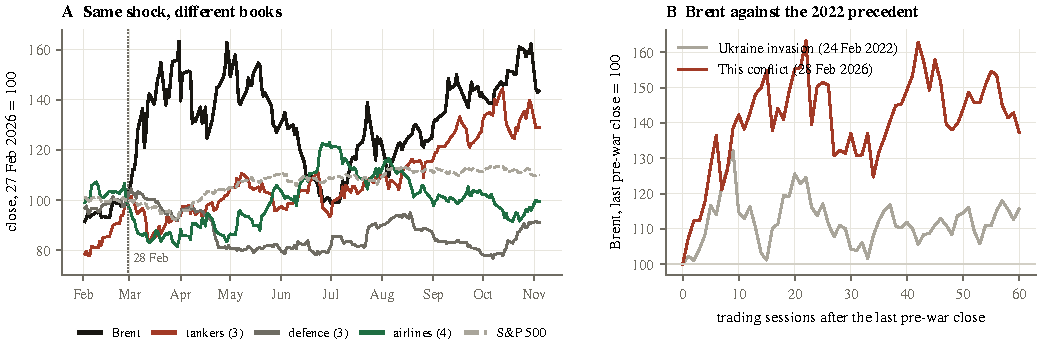
\includegraphics[width=\textwidth]{../figures/fig_markets.pdf}
\caption{\textbf{Money spoke on the first day.} (A) Closes normalised to 27 February 2026 = 100: oil, tankers, defence, airlines and equities moved very differently after 28 February. (B) Brent after the last pre-war close, here against the first sessions after Russia's 2022 invasion of Ukraine. Front-month futures; roll days can add small jumps.}\label{fig:markets}
\end{figure*}

\begin{table*}[t]
\centering\small
\caption{Change in close from the last pre-war session (27 February 2026). Daily closes from Yahoo Finance \citep{yahoofinance}; the peak column is the date of Brent's highest close (31 March).}\label{tab:markets}
\begin{tabular}{@{}lrrrrrr@{}}\toprule
Asset & 27 Feb & 2 Mar & +5 & +20 & Peak & 4 Nov\\
 & close & \multicolumn{5}{c}{change from 27 Feb close, \%}\\\midrule
Brent & 72.48 & $+$7.3 & $+$27.9 & $+$55.3 & $+$63.3 & $+$43.6\\
WTI & 67.02 & $+$6.3 & $+$35.6 & $+$48.7 & $+$51.3 & $+$43.8\\
TTF natural gas & 31.96 & $+$39.3 & $+$67.0 & $+$69.5 & $+$58.8 & $+$186.6\\
Gold & 5,247.90 & $+$1.2 & $-$1.7 & $-$14.4 & $-$11.4 & $-$23.2\\
S\&P 500 & 6,878.88 & 0.0 & $-$2.0 & $-$7.4 & $-$5.1 & $+$10.0\\
VIX & 19.86 & $+$8.0 & $+$48.5 & $+$56.3 & $+$27.1 & $+$4.9\\
Delta & 65.70 & $-$2.2 & $-$10.2 & $-$1.3 & $+$1.2 & $+$26.8\\
United & 106.30 & $-$2.9 & $-$13.4 & $-$16.8 & $-$13.4 & $+$0.9\\
Lufthansa & 9.09 & $-$5.2 & $-$10.7 & $-$19.1 & $-$20.8 & $-$17.8\\
Air France--KLM & 12.30 & $-$9.4 & $-$18.0 & $-$28.9 & $-$30.4 & $-$11.5\\
Frontline & 37.95 & $+$4.4 & $-$8.9 & $-$11.3 & $-$8.1 & $+$38.2\\
International Seaways & 75.53 & $+$1.3 & $-$4.1 & $-$5.8 & $-$3.5 & $+$38.7\\
A.P.~M{\o}ller--Maersk & 15,675.00 & $+$7.9 & $+$9.1 & $+$2.7 & $+$2.4 & $+$46.7\\
Lockheed & 658.08 & $+$2.8 & $+$2.1 & $-$6.4 & $-$8.2 & $-$2.9\\
Northrop & 724.38 & $+$6.0 & $+$4.4 & $-$6.3 & $-$5.8 & $-$24.0\\
\bottomrule\end{tabular}
\end{table*}

\paragraph{An audit of our own annotation.}
The dashboard carried a hand-written milestone: ``4 March 2026, Oil spikes \$\AuditClaim: Brent crude surges past \$\AuditClaim/bbl.'' The data say otherwise. Brent closed at \$\AuditClose\ that day (Yahoo reports the same value for 3 March, so the exact figure may be a repeated print; either way no session came near \$\AuditClaim). Its highest intraday price of the year was \$\AuditHigh\ (\AuditHighDate), and it never reached \$\AuditClaim\ in any session. The annotation was off by about \$59 and had been public for months. We have corrected it. The lesson is general: a curated annotation is a claim, and claims need the same audit as sensors.

\subsection{The ports went quiet}
Prices say something happened. Port calls say where. Inside the Persian Gulf, nine ports averaged \GulfPre\ calls a day before the war and \GulfPost\ after: \GulfRatio\pct\ of the earlier rate (95\pct\ CI \GulfLo--\GulfHi\pct; Table~\ref{tab:ports}, Fig.~\ref{fig:ports}). Tanker calls fell the same way, from \GulfTankPre\ to \GulfTankPost\ a day. Control ports did not move (\CtrlRatio\pct). On the Gulf of Oman coast, outside the strait, calls fell less (\OmanRatio\pct). The Eastern Mediterranean stayed near normal (\MedRatio\pct).

The path matters as much as the average. Inside-Gulf calls dropped to \GulfMar\pct\ of baseline in March, bottomed at \GulfMay\pct\ in May, recovered to \GulfJul\pct\ in July, and sat at \GulfOct\pct\ in October. The strait did not close and reopen; it narrowed and stayed narrow.

The Red Sea group tells a different story, and one we do not yet understand. Averaged over the whole post-window it held at \RedRatio\pct\ (CI \RedLo--\RedHi\pct), but it did not fall in March; it fell from August, to \RedOct\pct\ in October. One port drives this: Jeddah went from \JeddahJun\pct\ of baseline in June to \JeddahOct\pct\ in October, while Djibouti and Port Said stayed roughly flat; without Jeddah the group sits at \RedExJeddah\pct. A single-port collapse can be real or can be a change in how satellites count; we flag it and leave it open.

Independent evidence agrees on the Gulf. The U.S.\ Energy Information Administration reports oil flows through the Strait of Hormuz of 21.6 million barrels a day in the fourth quarter of 2025, 14.9 in the first quarter of 2026 and 4.9 in the second \citep{eia2026steo}. Hormuz normally carries about a fifth of the world's petroleum liquids \citep{eia2025hormuz}. Crucially, EIA adds that since the end of February ``AIS signal data for ships transiting the Strait of Hormuz have become especially unreliable'' \citep{eia2026steo}. Part of any AIS-based drop could therefore be lost signal rather than lost ships. We cannot separate the two. What we can say is that the port calls, the EIA flows, the oil price and the tanker equities all point the same way, and that no single one of them is pure.

\begin{figure*}[t]
\centering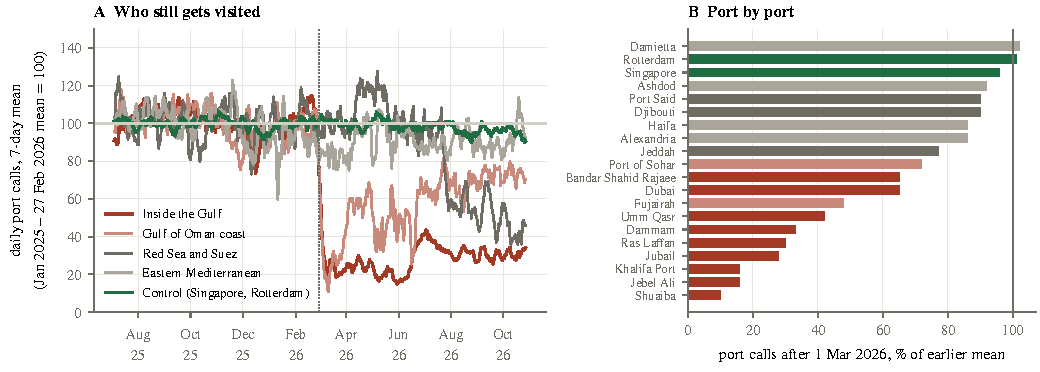
\includegraphics[width=\textwidth]{../figures/fig_ports.pdf}
\caption{\textbf{Ships that still call.} (A) Daily port calls, 7-day mean, as a share of each group's January 2025 to 27 February 2026 mean. The dotted line marks 28 February 2026. (B) Port-by-port ratio of calls after 1 March 2026 to calls before. Source: IMF PortWatch \citep{portwatch}.}\label{fig:ports}
\end{figure*}

\begin{table}[t]
\centering\small
\caption{Port calls per day before (1 Jan 2025--27 Feb 2026) and after (1 Mar--30 Oct 2026) the start of the conflict, with moving-block bootstrap intervals for the ratio.}\label{tab:ports}
\begin{tabular}{@{}lrrcc@{}}\toprule
Port group & Before & After & Ratio & 95\% CI\\
 & \multicolumn{2}{c}{calls per day} & & \\\midrule
Inside the Gulf & 74.3 & 20.9 & 0.28 & 0.26--0.30\\
Gulf of Oman coast & 16.9 & 9.7 & 0.57 & 0.52--0.63\\
Red Sea and Suez & 14.7 & 12.1 & 0.83 & 0.73--0.92\\
Eastern Mediterranean & 30.6 & 27.7 & 0.91 & 0.87--0.94\\
Control: Singapore, Rotterdam & 209.1 & 205.0 & 0.98 & 0.97--0.99\\
\bottomrule\end{tabular}
\end{table}

\subsection{The free ship feed is blind where it matters}
The most natural way to ask ``do ships still move through Hormuz?'' is to look at ship positions. We did. On 4 November 2026 the open global AIS snapshot held \AisTotal\ vessels. Only \AisFresh\ (\AisFreshPct\pct) had reported within the previous six hours; the median position was \AisMedianAge\ hours old and the ninetieth percentile \AisPnineAge\ hours (Fig.~\ref{fig:ais}, Table~\ref{tab:ais}). Repeated snapshots over \AisSpanMin\ minutes gave the same share (\AisFreshMin--\AisFreshMax\pct, $n=\AisSnaps$).

In the Strait of Hormuz box the snapshot held \HormuzAll\ vessels, of which \HormuzFresh\ were fresh. In the Persian Gulf, \PGulfAll\ vessels and \PGulfFresh\ fresh. In the Red Sea and at Bab el-Mandeb, \emph{no} vessel at any age. A careless reading says shipping stopped. But the Strait of Malacca, a busy and unthreatened lane, shows \MalaccaFresh\ fresh positions among \MalaccaAll\ (\MalaccaFreshPct\pct), while the North Sea shows \NSeaFreshPct\pct. The Gulf is quieter than any other lane we measured. That fits lost ships, jammed signals or a thin receiver network, and one snapshot cannot say which. The Red Sea's zero at every age looks more like a filter in the provider's feed than silence at sea. For this question the open ship feed is not enough on its own; the port calls above are a better check, though not an independent one, since they too derive from AIS.

This is a finding about our own dashboard too. Its vessel layer draws every position in the snapshot, including positions that are days or months old. We now label that layer by age rather than let stale ships pose as live ones.

\begin{figure*}[t]
\centering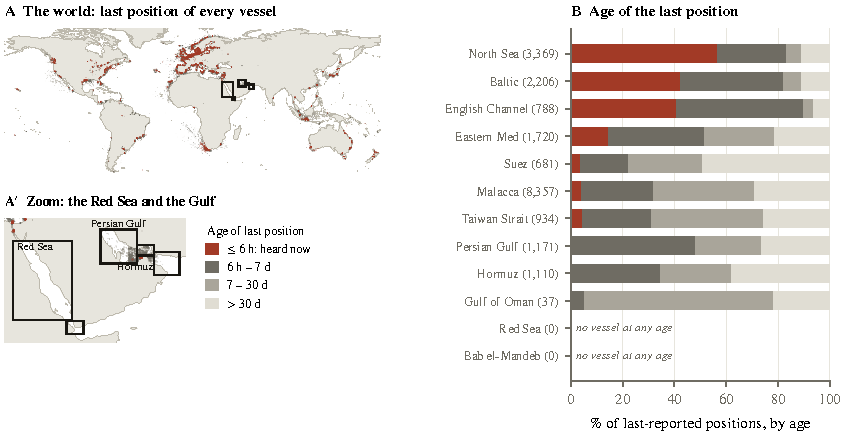
\includegraphics[width=\textwidth]{../figures/fig_ais.pdf}
\caption{\textbf{Observability of open ship data.} (A) \AisTotal\ vessel positions from the Axiom Overwatch snapshot \citep{overwatch}, 4 November 2026, coloured by age. Fresh positions (red) are densest in northern Europe, with fewer in Asia and North America. Boxes: Hormuz, Persian Gulf, Gulf of Oman, Bab el-Mandeb, Red Sea. (B) Share of last-reported positions by age in each analysis box; counts in brackets.}\label{fig:ais}
\end{figure*}

\begin{table}[t]
\centering\small
\caption{Last-reported vessel positions in analysis boxes (first snapshot, 4 Nov 2026, 07:07 UTC). ``Fresh'' means reported within six hours.}\label{tab:ais}
\begin{tabular}{@{}lrrrr@{}}\toprule
Box & Vessels & $\le$6\,h & \% fresh & Median age\\
 & (any age) & (n) & & (hours)\\\midrule
North Sea & 3,369 & 1,914 & 56.8 & 1\\
Baltic & 2,206 & 936 & 42.4 & 19\\
Eastern Med & 1,720 & 248 & 14.4 & 153\\
Suez & 681 & 26 & 3.8 & 536\\
Malacca & 8,357 & 353 & 4.2 & 314\\
Taiwan Strait & 934 & 41 & 4.4 & 376\\
Persian Gulf & 1,171 & 1 & 0.1 & 173\\
Hormuz & 1,110 & 0 & 0.0 & 279\\
Gulf of Oman & 37 & 0 & 0.0 & 366\\
Red Sea & 0 & 0 & -- & --\\
Bab el-Mandeb & 0 & 0 & -- & --\\
\bottomrule\end{tabular}
\end{table}

\subsection{The sky, and the regulator}
Aircraft are harder to hide and easier to lose. We sampled airborne ADS-B aircraft over a box covering the Middle East ($10$--$42^\circ$N, $24$--$65^\circ$E) and two control boxes, Europe and Southeast Asia, \AirN\ times on 4 November 2026 (Fig.~\ref{fig:air}, Table~\ref{tab:air}). The Middle East box held \AirME\ airborne aircraft per sample on average (range \AirMELo--\AirMEHi), Europe \AirEU\ and Southeast Asia \AirSEA. Per unit of land area the United Arab Emirates was the busiest airspace in the box (\DensUAE\ aircraft per 100\,000\,km\textsuperscript{2}, above the European median of \AirEUMedian), followed by a cluster of small, well-covered countries (Georgia, Israel and Greece). Iran (\DensIran), Iraq (\DensIraq) and Yemen read close to zero.

These are the countries for which the European Union Aviation Safety Agency (EASA) currently advises caution (Table~\ref{tab:czib}). The regulator's own clock is a witness. A bulletin for ``Iran and neighbouring airspace'' was first issued on 16 January 2026, six weeks before the war. A region-wide bulletin for the Middle East and the Persian Gulf was issued on 28 February, the day of the first strikes, was revised fourteen times, and was last revised on 1 July (valid to 8 July). Country bulletins followed: Iran, Iraq and Lebanon on 8 July, the Persian Gulf and Gulf of Oman on 14 July, Jordan on 22 July, and Saudi Arabia as late as 30 September \citep{easa2026czib}. The advice was reissued country by country as the region-wide bulletin retired.

But look at Egypt. Egypt has no active bulletin, yet it reads almost as empty as Iraq (\DensEgypt\ against \DensIraq\ aircraft per 100\,000\,km\textsuperscript{2}). That is not a closed sky; it is a sky the open receivers cannot hear. So an empty cell is a question, not an answer. Aircraft density is only a weak check on the regulator: countries with a bulletin, such as Jordan and Syria, sit beside countries with none, such as Turkey and Georgia, and it says little where receivers are thin.

\begin{figure*}[t]
\centering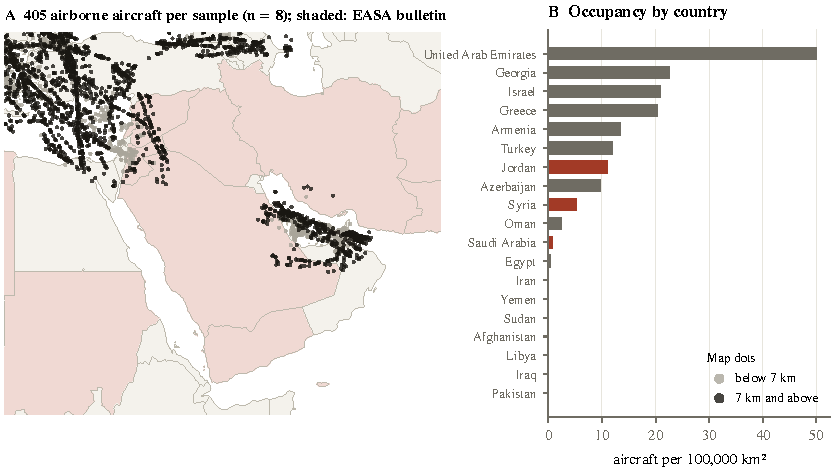
\includegraphics[width=\textwidth]{../figures/fig_air.pdf}
\caption{\textbf{The sky over the Middle East.} (A) Airborne ADS-B aircraft pooled over all samples on 4 November 2026 (OpenSky \citep{opensky}); countries with an active EASA bulletin are shaded. Dark points are at or above 7\,km. (B) Mean aircraft per 100\,000\,km\textsuperscript{2} of country area inside the sampled box. Egypt, with no bulletin, reads almost as empty as Iraq: coverage, not closure, dominates the lowest bars.}\label{fig:air}
\end{figure*}

\begin{table*}[t]
\centering\small
\caption{EASA Conflict Zone Information Bulletins relevant to the conflict, as listed on 4 November 2026 \citep{easa2026czib}. $^\dagger$Withdrawn. Dates as shown on the page: issue, last revision, valid until.}\label{tab:czib}
\begin{tabular}{@{}llccc@{}}\toprule
Airspace & Reference & Issued & Revised & Valid until\\\midrule
Iran and neighbouring airspace$^\dagger$ & 2026-02-R1 & 16 Jan 2026 & 12 Feb 2026 & 31 Mar 2026\\
Middle East and Persian Gulf$^\dagger$ & 2026-03-R14 & 28 Feb 2026 & 1 Jul 2026 & 8 Jul 2026\\
Lebanon & 2026-06-R2 & 8 Jul 2026 & 30 Sep 2026 & 16 Nov 2026\\
Iraq & 2026-05-R2 & 8 Jul 2026 & 30 Sep 2026 & 16 Nov 2026\\
Iran & 2026-04-R2 & 8 Jul 2026 & 30 Sep 2026 & 16 Nov 2026\\
Persian Gulf and Gulf of Oman & 2026-07R3 & 14 Jul 2026 & 30 Sep 2026 & 16 Nov 2026\\
Jordan & 2026-08-R3 & 22 Jul 2026 & 14 Oct 2026 & 16 Nov 2026\\
Saudi Arabia & 2026-09-R1 & 30 Sep 2026 & 9 Oct 2026 & 16 Nov 2026\\
\bottomrule\end{tabular}
\end{table*}

\begin{table}[t]
\centering\small
\caption{Airborne ADS-B aircraft per sample by country inside the Middle East box (countries over 20\,000\,km\textsuperscript{2}; area clipped to the box).}\label{tab:air}
\begin{tabular}{@{}lrrrr@{}}\toprule
Country & Area & Mean & per & EASA\\
 & (km$^2$) & aircraft & 100\,000\,km$^2$ & bulletin\\\midrule
United Arab Emirates & 71,443 & 35.8 & 50.0 & no\\
Georgia & 30,443 & 6.9 & 22.6 & no\\
Israel & 22,103 & 4.6 & 20.9 & no\\
Greece & 29,995 & 6.1 & 20.4 & no\\
Armenia & 29,625 & 4.0 & 13.5 & no\\
Turkey & 781,404 & 93.6 & 12.0 & no\\
Jordan & 89,074 & 9.8 & 10.9 & yes\\
Azerbaijan & 86,605 & 8.4 & 9.7 & no\\
Syria & 186,430 & 9.9 & 5.3 & yes\\
Oman & 312,975 & 7.8 & 2.5 & no\\
Saudi Arabia & 1,934,022 & 13.0 & 0.7 & yes\\
Egypt & 1,006,994 & 4.6 & 0.5 & no\\
Iran & 1,629,383 & 0.6 & 0.0 & yes\\
Pakistan & 130,781 & 0.0 & 0.0 & yes\\
Iraq & 438,711 & 0.0 & 0.0 & yes\\
Libya & 128,668 & 0.0 & 0.0 & yes\\
Afghanistan & 262,421 & 0.0 & 0.0 & yes\\
Sudan & 1,734,703 & 0.0 & 0.0 & yes\\
Yemen & 455,299 & 0.0 & 0.0 & yes\\
\bottomrule\end{tabular}
\end{table}

\subsection{What burns}
Thermal satellites see heat, not intent. The open FIRMS file for \FirmsFrom\ to \FirmsTo\ held \FirmsRows\ global detections over \FirmsDays\ days. The first task is to separate chronic sources from transient ones: in the Persian Gulf basin \FirmsGulfChronic\pct\ of the \FirmsGulfCells\ detected 1\,km cells lit up on at least two-thirds of the days, against at most \FirmsOtherChronicMax\pct\ in Ukraine, Sudan, Myanmar, the Levant or western Europe (Fig.~\ref{fig:fire}). That is consistent with industrial flaring, which is why a single bright pixel at a Gulf oil terminal says almost nothing on its own. Only \FirmsGulfBig\ transient cells in the basin exceeded 50\,MW in the window. We report them as candidates, not events; we have no ground truth. Measuring \emph{environmental damage} (smoke plumes, spills, burned land) needs imagery and a baseline we do not yet have, though earlier wars show what is possible \citep{hobbs1992kuwait,unep2024gaza}.

\begin{figure}[t]
\centering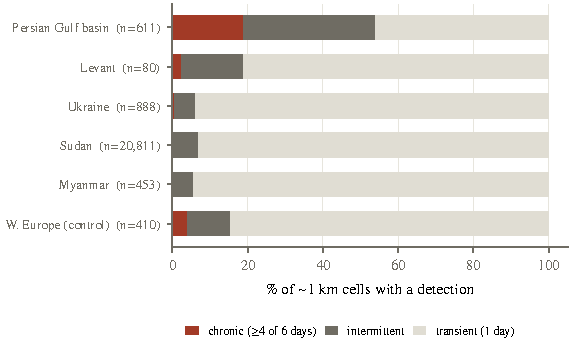
\includegraphics[width=\columnwidth]{../figures/fig_fire.pdf}
\caption{\textbf{Chronic or transient.} Share of detected 1\,km cells by number of days lit, by region, from the FIRMS 7-day file \citep{firms,schroeder2014viirs}. The Gulf basin shows the chronic signature of flares.}\label{fig:fire}
\end{figure}

\subsection{An audit of the observatory itself}
Table~\ref{tab:audit} shows the state of our own feeds on audit day. Four of ten data feeds were down or demonstration-only: one had no key and returned an empty payload by design, one served clearly labelled demonstration events, and two had upstream errors. A fifth, the ship feed, was live but stale. One composite output deserves a second look. The platform's escalation gauge read 2 out of 100, ``LOW'', on a day when Brent stood at \$\BrentLatest. The score was computed from three inputs that were offline (heat, news, strikes) and one that was live (markets), and the system knew it: its own field said only 25 of 100 points were available. The display did not say so. We call this a \emph{false calm}. A broken pipe looks exactly like peace unless the instrument is made to tell the difference, and the reader of a map cannot tell which they are looking at.

\begin{table}[t]
\centering\small
\caption{State of the platform's own feeds on 4 November 2026, 07:00 UTC.}\label{tab:audit}
\begin{tabular}{@{}>{\raggedright\arraybackslash}p{2.05cm}>{\raggedright\arraybackslash}p{1.3cm}>{\raggedright\arraybackslash}p{4.1cm}@{}}
\toprule
Feed & State & Note\\\midrule
Markets, oil & live & Yahoo Finance; platform feed, 129 sessions\\
Flights & live & adsb.lol (platform feed); 134 in the Middle East box\\
Quakes, UNHCR & live & USGS; UNHCR displacement\\
Ships & stale & live feed, but 82.5\pct\ of positions older than 6\,h\\
Heat (FIRMS) & offline & key not set; empty by design\\
Conflict events & demo & labelled \texttt{demo\_offline}\\
News sentiment & error & upstream HTTP 502\\
Maritime warnings & error & upstream HTTP 503\\
Escalation gauge & misleading & 2/100 ``LOW'' from 1 of 4 inputs\\\bottomrule
\end{tabular}
\end{table}

\section{Discussion}
\subsection{Did we see better than the journalists?}
No, and it would be a mistake to say so. A reporter can ask a question, smell smoke and meet a family. We cannot. What we can do is different, and three things stand out. We see a whole sea at once, which no reporter can. We see \emph{absence over time}, such as ports that quietly fell to a fraction of their traffic, which no single story records. And we see money's verdict, which is a vote by people with something to lose.

Equally, three things are out of reach: \emph{why} (a falling port count does not say whether the cause was mines, insurance or fear), \emph{who} (a transient thermal cell does not say whose weapon), and the human cost, which is the reason the question matters at all.

\subsection{The strongest objection}
The best counter-argument runs as follows. Sensors are contested terrain. Ships switch transponders off; signals can be jammed or spoofed; receivers are placed by volunteers, who are not placed evenly across a war. A platform that shows sensor data with confidence may mislead more than a hesitant reporter, because a map looks like truth. The objection is right, and our own results illustrate it: the free ship feed cannot hear the Gulf, the aircraft feed cannot hear Egypt, and our own dashboard once drew days-old ships as live.

\subsection{What survives}
What survives is a principle. \emph{Treat every channel as a witness with known eyesight, and print the eyesight next to the testimony.} Concretely: (1) show the age of every position and the coverage of every region beside the data; (2) refuse a composite score when its inputs are missing, and say ``insufficient data'' instead of ``low''; (3) triangulate across witnesses that fail for different reasons, such as ports, flows, prices and regulators; (4) record the provenance of every hand-written annotation and audit it like a sensor; (5) keep it free and open, so that anyone can repeat the audit. This is a design rule, not a technology. It costs nothing to implement and it changes what the screen claims.

\subsection{Ethics and safety}
Every input is already public, and our analyses use aggregate counts; we do not follow named people, vessels or aircraft over time. The dashboard displays only what its sources publish. Open tools can help the careful and the careless alike, so we recommend that deployments avoid persistent tracks of individual military assets and avoid alerts keyed to named facilities. We do not describe any use as targeting. Our figures about journalists come from CPJ, whose counts it revises as cases are reviewed \citep{cpj2026report,cpj2025report}.

\section{Limitations}
This is one event over eight months, not years: the platform's continuous archive was not retained, so the longitudinal evidence comes from public series that can be reconstructed (prices, port calls, regulator bulletins), and the ship, aircraft and heat results are cross-sections on a single day. The aircraft result rests on \AirN\ samples from an anonymous research API with uneven coverage. Port calls are model estimates from satellite AIS, and the source flags the Gulf as unreliable \citep{eia2026steo}. The Yahoo Finance endpoint is unofficial and its terms restrict some uses, so we archive derived closes only. Front-month futures contain roll jumps. Geography fixed the port groups, but their size is small. The bulletins list is a snapshot of a page that changes weekly. We found no way to test our results against ground truth on casualties or damage, and we make no claim about either.

\section{Conclusion}
A war can be partly seen from a laptop. The money spoke on the first day and spoke hard. Ports inside the Persian Gulf fell to under a third of their usual traffic and stayed low. The regulator reissued its advice country by country. These readings agree, and they come from witnesses that fail for different reasons, which is why we trust them. The same method told us that the free ship feed cannot hear the Gulf, that the aircraft feed cannot hear Egypt, and that our own dashboard had said things that were not true. The lesson is not to look harder. It is to say, beside every number, how well we could have heard.

\section*{Data and code availability}\label{sec:avail}
The platform, analysis scripts, derived tables and this paper's \LaTeX\ source are in the repository \href{https://github.com/Nonarkara/globalmonitor-v3}{github.com/Nonarkara/globalmonitor-v3} under \texttt{research/} (MIT licence). Source data keep their original licences: PortWatch, OpenSky, adsb.lol, Axiom Overwatch (CC-BY~4.0), NASA FIRMS, EASA, EIA, Natural Earth \citep{naturalearth}. Live URL: \href{https://globalmonitor.nonarkara.org}{globalmonitor.nonarkara.org}.

\section*{Funding and competing interests}
The platform is supported by the Program Management Unit for Area Based Development (PMU A) and the Digital Economy Promotion Agency (depa), and executed by Axiom and The Reason to Live Company (ReTL). The corresponding author works at depa, one of the funders; readers should weigh the results accordingly. The ship snapshot comes from a service named Axiom Overwatch, and Axiom executes the platform; treat that feed as not independent of this project.

\bibliographystyle{plainnat}
\bibliography{references}
\end{document}
